\chapter{測量、密度矩陣與熵}

雙縫實驗以最精簡而仍有用的形式呈現測量問題。兩種可能性保持相干時，它們的振幅會相互干涉；另一個系統一旦留下粒子所經路徑的記錄，粒子便與記錄器糾纏，干涉也會因此改變。在引入跡、密度矩陣與熵---這些量化糾纏所需的概念之前，我們先精確說明這個機制。

\section{重新建構雙縫實驗}

考慮一個離散模型：源位於格點\(0\)，兩個開口位於\(A\)與\(B\)，螢幕上可能的到達位置以正交歸一態\(\{|m\rangle\}\)表示。粒子可以是電子、光子或任何其他量子物體。我們稱它為電子，並忽略電子本身的自旋，因此這裡只討論位置這個自由度。障壁的其餘部分都是封閉的：電子若到達\(A\)或\(B\)以外的任何格點，就會被反射。

線性是這裡的結構原理。若兩個態的演化如下：
\begin{equation}
|A\rangle\longrightarrow |A'\rangle,
\qquad
|B\rangle\longrightarrow |B'\rangle,
\end{equation}
則任何疊加態也會以相同的係數演化：
\begin{equation}
\alpha|A\rangle+\beta|B\rangle
\longrightarrow
\alpha|A'\rangle+\beta|B'\rangle.
\end{equation}

在對稱的配置中，源以相同振幅向兩個開口傳播。和黑板上一樣，省略共同的歸一化因子：
\begin{equation}
|0\rangle\longrightarrow |A\rangle+|B\rangle.
\end{equation}
歸一化後的態應為\((|A\rangle+|B\rangle)/\sqrt{2}\)；省略的因子不影響干涉論證。

現在分別考察每一條路徑。從開口傳播到螢幕的形式為
\begin{align}
|A\rangle &\longrightarrow \sum_m \psi_m|m\rangle, \\
|B\rangle &\longrightarrow \sum_m \phi_m|m\rangle.
\end{align}
複數\(\psi_m\)表示粒子從\(A\)出發後到達螢幕格點\(m\)的振幅；\(\phi_m\)則表示從\(B\)出發後到達該處的振幅。

\begin{figure}[htbp]
\centering
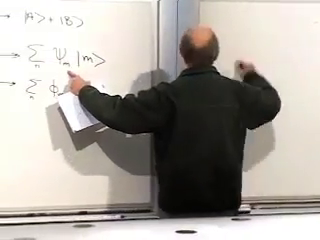
\includegraphics[width=0.68\textwidth]{lecture_07_figure_02.png}
\caption{在螢幕基底下，分別沿\(A\)路徑與\(B\)路徑展開。}
\lectureframe{00:05:39}
\end{figure}

若關閉\(B\)，則粒子在\(m\)處的機率為
\begin{equation}
P_A(m)=|\psi_m|^2.
\end{equation}
若關閉\(A\)，則
\begin{equation}
P_B(m)=|\phi_m|^2.
\end{equation}
依照古典機率，兩個開口都開啟時，應將上述兩個結果相加。但量子力學是先將振幅相加：
\begin{equation}
|A\rangle+|B\rangle
\longrightarrow
\sum_m(\psi_m+\phi_m)|m\rangle.
\end{equation}
在螢幕上的固定格點處，
\begin{align}
P(m)
&=|\psi_m+\phi_m|^2 \\
&=|\psi_m|^2+|\phi_m|^2
  +\psi_m^*\phi_m+\phi_m^*\psi_m.
\end{align}

\begin{figure}[htbp]
\centering
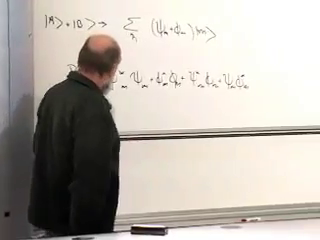
\includegraphics[width=0.70\textwidth]{lecture_07_figure_03.png}
\caption{螢幕位置的機率展開為四項，最後兩項是干涉項。}
\lectureframe{00:09:21}
\end{figure}

在對稱點上，\(\psi_m=\phi_m\)，兩種可能性會相長干涉。在兩者相位相差\(\pi\)的點上，\(\psi_m=-\phi_m\)，機率為零。單獨考慮任一條路徑，粒子都能到達該點；但兩條路徑同時開啟時，電子反而可能無法到達那裡。於是，一個無可迴避的問題浮現了：當某個東西記錄了電子經過哪個開口時，會有什麼改變？

\section{探測器與系統糾纏}

引入一個輔助的二態系統，其狀態為\(|u\rangle\)與\(|d\rangle\)。在這個模型中，它不是電子的自旋，而是一個最簡單的外部裝置。初始時，探測器尚未觸發：
\begin{equation}
|0,d\rangle.
\end{equation}
安排相互作用，使電子通過\(A\)時探測器翻轉，通過\(B\)時則維持原狀：
\begin{equation}
|0,d\rangle
\longrightarrow
|A,u\rangle+|B,d\rangle.
\end{equation}
電子離開開口後，不再與輔助自旋相互作用。因此，兩個分支分別演化為
\begin{align}
|A,u\rangle &\longrightarrow \sum_m\psi_m|m,u\rangle, \\
|B,d\rangle &\longrightarrow \sum_m\phi_m|m,d\rangle,
\end{align}
最後的狀態為
\begin{equation}
|\Psi\rangle
=\sum_m\left(\psi_m|m,u\rangle+\phi_m|m,d\rangle\right).
\end{equation}
此時路徑已與探測器的記錄糾纏。讀取探測器就能得知電子經過哪個開口。

\begin{classroomqa}
\lecturetimestamp{00:13:24}
\audiencequestion{自旋翻轉時，波包是否已經坍縮？}
\lecturerresponse{只考慮電子時，可以用坍縮來描述：各路徑的可能性已不再互相干涉。然而，對完整的電子--探測器系統而言，兩個分支都沒有被捨棄，狀態仍是\(|A,u\rangle+|B,d\rangle\)。若把裝置也納入描述，就能以更精確的說法取代\emph{電子已經坍縮}：系統--裝置之間已建立糾纏。}
\end{classroomqa}

輔助自旋只是方便使用的指標。無論是裝置觸發或未觸發、光子發射或未發射，或其他任何一對可區分的記錄，都能扮演相同的角色。

\begin{classroomqa}
\lecturetimestamp{00:15:17}
\audiencequestion{電子穿過金屬板時，金屬板一定會留下路徑記錄嗎？}
\lecturerresponse{不一定。關鍵在於相互作用是否使金屬板處於可區分的末態。若金屬板有激發能隙，而電子的能量不足以激發它，就不一定會留下持續存在的內部標記。光有相互作用還不夠；兩種可能性必須分別與可區分的記錄相關聯。}
\end{classroomqa}

\begin{classroomqa}
\lecturetimestamp{00:16:29}
\audiencequestion{金屬板的反衝能否揭示電子是通過上方還是下方的開口？}
\lecturerresponse{只有當方向相反的動量衝擊使金屬板處於足夠可區分的狀態時，才有可能。位置高度局域的金屬板，其動量波函數本來就很寬。微小的向上與向下位移可能幾乎完全重疊，因此反衝後的狀態並不正交，無法提供明確的路徑記錄。這正是不確定性原理保護干涉的地方。}
\end{classroomqa}

部分記錄是可能的。若探測器只受到輕微的推動，兩個最終記錄態不一定正交。此時干涉會減弱，但不會完全消失。為了進行形式上的計算，我們先考慮完全測量的極限情況：
\begin{equation}
\langle u|d\rangle=0.
\end{equation}

\section{投影算符的計算}

現在計算電子到達螢幕固定位置\(m\)的機率，不考慮探測器的測量結果。在合併後的希爾伯特空間中，性質\emph{電子位於\(m\)}所對應的是一個二維子空間，由下列態張成：
\begin{equation}
|m,u\rangle,\qquad |m,d\rangle.
\end{equation}
相應的投影算符為
\begin{equation}
\Pi_m
=|m,u\rangle\langle m,u|
 +|m,d\rangle\langle m,d|.
\end{equation}

\begin{figure}[htbp]
\centering
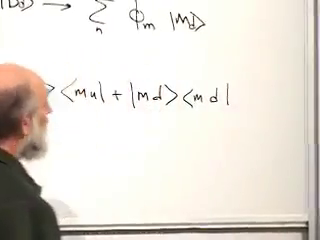
\includegraphics[width=0.66\textwidth]{lecture_07_figure_04.png}
\caption{投影到螢幕上的固定位置，並對兩個正交的探測器記錄求和。}
\lectureframe{00:22:04}
\end{figure}

根據機率公設，
\begin{equation}
P(m)=\langle\Psi|\Pi_m|\Psi\rangle.
\end{equation}
將求和展開後，
\begin{align}
P(m)
&=
\sum_{n,n'}
\left(\psi_n^*\langle n,u|+\phi_n^*\langle n,d|\right)
\notag\\
&\quad\times\Pi_m
\notag\\
&\quad\times
\left(\psi_{n'}|n',u\rangle+\phi_{n'}|n',d\rangle\right).
\end{align}
位置的內積要求\(n=m=n'\)。接著由探測器的內積決定哪些項會保留下來：
\begin{align}
\langle u|u\rangle&=1,
&
\langle d|d\rangle&=1,
&
\langle u|d\rangle&=\langle d|u\rangle=0.
\end{align}
因此，
\begin{equation}
P(m)=|\psi_m|^2+|\phi_m|^2.
\end{equation}

交叉項並非被任意規定為零。它們之所以消失，是因為兩條路徑的振幅現在分別乘上擴大的狀態空間中互相正交的向量。若要產生干涉，各種可能性不只必須在螢幕端點相同，凡是會留下記錄的自由度也都必須一致。

\section{什麼情況才算測量？}

這個簡明的自旋模型給出一條一般原則：當相互作用使系統的不同可能性與裝置的可區分狀態建立關聯時，測量便發生了。以下幾種變化可以檢驗這條原則。

\begin{classroomqa}
\lecturetimestamp{00:26:53}
\audiencequestion{如果把自旋對稱地放置，讓它在電子通過任一開口時都翻轉，會怎麼樣？}
\lecturerresponse{那麼兩個分支帶有相同的記錄\(|A,u\rangle+|B,u\rangle=(|A\rangle+|B\rangle)\otimes|u\rangle\)。探測器的狀態可以因式分解出來，並未揭露任何路徑資訊，因此干涉圖樣仍會保留。}
\end{classroomqa}

\begin{figure}[htbp]
\centering
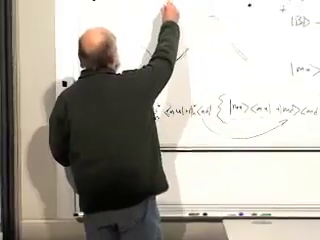
\includegraphics[width=0.68\textwidth]{lecture_07_figure_05.png}
\caption{黑板上的另一種配置：探測器對稱放置，對兩條路徑的反應相同。}
\lectureframe{00:27:14}
\end{figure}

\begin{figure}[htbp]
\centering
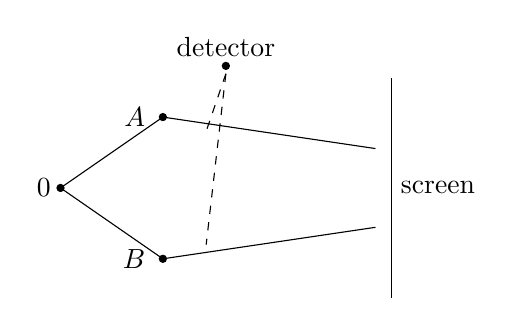
\begin{tikzpicture}[scale=1.0]
\fill (-2,0) circle (1.5pt);
\node[left] at (-2,0) {$0$};
\fill (-0.7,0.9) circle (1.5pt);
\node[left] at (-0.8,0.9) {$A$};
\fill (-0.7,-0.9) circle (1.5pt);
\node[left] at (-0.8,-0.9) {$B$};
\draw (-2,0) -- (-0.7,0.9);
\draw (-2,0) -- (-0.7,-0.9);
\draw (-0.7,0.9) -- (2.0,0.5);
\draw (-0.7,-0.9) -- (2.0,-0.5);
\draw (2.2,-1.4) -- (2.2,1.4);
\node[right] at (2.2,0) {screen};
\fill (0.1,1.55) circle (1.5pt);
\node[above] at (0.1,1.55) {detector};
\draw[dashed] (0.1,1.45) -- (-0.15,0.72);
\draw[dashed] (0.1,1.45) -- (-0.15,-0.72);
\end{tikzpicture}
\caption{對稱放置探測器的清楚重建：兩條路徑都會使探測器進入相同狀態。}
\end{figure}

\begin{classroomqa}
\lecturetimestamp{00:27:55}
\audiencequestion{干涉消失之前，必須有人實際讀取輔助自旋嗎？}
\lecturerresponse{不必。電子已經讓路徑與自旋彼此相關。可以重設探測器，一次發射一個電子重複實驗，只檢查螢幕上撞擊位置的分佈。即使沒有人讀取自旋，干涉條紋也已消失；起作用的是物理記錄，而非人是否察覺它。}
\end{classroomqa}

\begin{classroomqa}
\lecturetimestamp{00:29:36}
\audiencequestion{足夠輕的反衝金屬板會破壞干涉嗎？}
\lecturerresponse{會，若反衝使金屬板因兩條路徑而進入互相正交的動量態。若移動後的波包仍然重疊，干涉就只會部分消失。判準不是質量本身，而是金屬板末態是否可區分。}
\end{classroomqa}

輻射是另一種不完美的記錄方式。帶電粒子加速時可能發射光子。在\(A\)附近發射的輻射，未必與在\(B\)附近發射的輻射處於相同狀態，因此電磁場可能保留路徑資訊。電子若只是緩慢偏轉，發射機率可能很低；講課中舉例估計約每一百次事件才發生一次。加速度越大，越可能產生輻射，也越可能降低條紋對比。關鍵在於定性結論：即使光子沒有被觀測到，也能帶走相干性。

\begin{classroomqa}
\lecturetimestamp{00:32:00}
\audiencequestion{在對比度不完美的實驗中，如何推算干涉機率？}
\lecturerresponse{重複實驗許多次，再根據相對頻率估計螢幕上的分佈。樣本數有限，加上環境留下的記錄，會使名義上的暗區仍有少量計數。試驗次數越多，推算出的機率分佈越準確；退相干過程則會降低實際干涉條紋的對比度。}
\end{classroomqa}

\begin{classroomqa}
\lecturetimestamp{00:33:13}
\audiencequestion{只要有可能判定路徑，干涉就會完全消失嗎？}
\lecturerresponse{路徑完全可區分時，干涉才會完全消失；只能取得部分資訊時，干涉也只會部分減弱。若探測器只稍微旋轉，兩個記錄態仍不正交。讀取探測器後，可以判斷某條路徑較有可能，但不能確定；相應地，條紋會變模糊，而非完全消失。}
\end{classroomqa}

令\(|E_A\rangle\)與\(|E_B\rangle\)代表任意的記錄態。螢幕處的合併狀態可寫為
\begin{equation}
|\Psi\rangle
=\sum_m\left(
\psi_m|m\rangle|E_A\rangle
+\phi_m|m\rangle|E_B\rangle
\right).
\end{equation}
忽略記錄系統後，得到
\begin{align}
P(m)
&=|\psi_m|^2+|\phi_m|^2 \\
&\quad
+\psi_m^*\phi_m\langle E_A|E_B\rangle
+\phi_m^*\psi_m\langle E_B|E_A\rangle.
\end{align}
因此，重疊\(\langle E_A|E_B\rangle\)就是相干因子。兩種可能性留下相同記錄時，干涉完全保留；記錄互相正交時，干涉消失；重疊程度介於兩者之間時，可見度也介於兩者之間。

\begin{classroomqa}
\lecturetimestamp{00:34:12}
\audiencequestion{若只有偶爾才會發射光子，只保留有光子發射的事件時會怎麼樣？}
\lecturerresponse{這個選出的子系綜通常會有較弱的干涉，因為光子帶有路徑資訊。但干涉不一定完全消失：兩個開口發出的光子波包可能彼此重疊，因此輻射所留下的記錄也未必完全正交。}
\end{classroomqa}

環境的持續轟擊會放大這個機制。空氣分子、環境光子與周圍物質不斷記錄宏觀物體的位置。人或月球不會以可見的方式維持在位置相干疊加態中：質量會減緩自由展寬，而與環境持續糾纏，則會抑制宏觀分離的可能性之間可觀測到的干涉。

\begin{classroomqa}
\lecturetimestamp{00:36:02}
\audiencequestion{這已經是在提出測量理論，而不只是再次使用\emph{波包坍縮}這個說法嗎？}
\lecturerresponse{這是一個刻意精確的例子，用來展示其中的機制。只描述電子時，坍縮就是捨棄非對角的\(\psi^*\phi\)項；描述複合系統時，則不必任意刪去任何項：與正交的裝置狀態糾纏後，這些項便無法透過只測量電子來取得。更複雜的例子也應回到這個結構來理解。}
\end{classroomqa}

\begin{classroomqa}
\lecturetimestamp{00:38:04}
\audiencequestion{若引力場使路徑自然彎曲，輻射的論證或干涉規則會改變嗎？}
\lecturerresponse{輻射的細節可能改變；而在測量路徑之前，量子力學並不指定一條確定的軌跡。一般結論則不變：只有會保留可區分路徑資訊的自由度，才會抑制干涉。若要進一步詳細回答，就必須先指定具體的裝置。}
\end{classroomqa}

\begin{classroomqa}
\lecturetimestamp{00:39:44}
\audiencequestion{這種干涉與古典電磁波的干涉不同嗎？}
\lecturerresponse{對於許多光子，觀察到的圖樣與電磁場的普通波動干涉一致。單粒子實驗則展現更深一層的量子描述：光子與電子是一次一個地抵達，而它們的量子振幅會互相干涉。對電子而言，相關的波是電子波函數，不是電磁波。}
\end{classroomqa}

\begin{classroomqa}
\lecturetimestamp{00:40:45}
\audiencequestion{初始波中瞄準\(A\)與\(B\)之間的部分會怎麼樣？}
\lecturerresponse{在這個刻意採用的離散模型中，障壁的其餘部分都被封住。這些部分會被反射，不會對透射到螢幕的振幅有所貢獻。此模型只隔離出兩種透射可能性，並不表示真實光束只有兩個動量分量。}
\end{classroomqa}

\section{貓、螢幕與可移動的切分界線}

同樣的數學也適用於Schr\"odinger的貓。令槍的狀態\(|U\rangle\)與\(|F\rangle\)分別代表未擊發與已擊發，貓的狀態\(|L\rangle\)與\(|D\rangle\)則分別代表活著與死亡。從活貓與未擊發的槍開始，相互作用可能產生
\begin{equation}
|\Psi_{\mathrm{cat}}\rangle
=\alpha|L,U\rangle+\beta|D,F\rangle.
\end{equation}
單看貓，牠並未處於相干態\(\alpha|L\rangle+\beta|D\rangle\)。牠與已記錄下不同可能性的槍糾纏在一起。觀察槍可以得知貓所處的分支；槍的正交記錄則消除了貓子系統中一般的活--死干涉。

\begin{classroomqa}
\lecturetimestamp{00:41:18}
\audiencequestion{貓本身是否處於生與死的疊加態？}
\lecturerresponse{若按簡單的孤立系統來看，並非如此。貓--槍這個複合系統處於兩種彼此相關的可能性疊加中：槍未擊發時貓活著，槍擊發時貓死亡。貓這個子系統與帶有記錄的槍糾纏，正如電子的路徑與輔助自旋糾纏一樣。}
\end{classroomqa}

最終的螢幕也必須視為一種測量裝置。電子抵達\(m\)時，可能使照相乳劑中的一顆微粒變黑、使閃爍體發出光子，或使一排局部二態裝置中的某個探測器翻轉。這個標記便與電子的到達位置相關聯。

\begin{classroomqa}
\lecturetimestamp{00:43:38}
\audiencequestion{為什麼可以談論電子在最終螢幕上的機率，而不必永遠只描述態向量？}
\lecturerresponse{機率公設把\(\langle\Pi_m\rangle\)賦予「\emph{抵達\(m\)}」這項性質。要完成物理實驗，螢幕接著會留下位置記錄。投影算符給出機率；變黑、發出閃爍光或局部探測器翻轉，則實現了我們要收集其統計結果的測量。}
\end{classroomqa}

\begin{classroomqa}
\lecturetimestamp{00:45:00}
\audiencequestion{為什麼討論螢幕測量時，卻不討論通過\(A\)或\(B\)的機率？}
\lecturerresponse{只有設置路徑記錄器，才能賦予並檢驗路徑機率。若沒有這種記錄，各種可能性仍保持相干，必須先將振幅相加。至於螢幕處，則假設有一個能分辨位置的裝置。兩者的差別不在於某個特殊時刻，而在於是否安排了相應的測量交互作用。}
\end{classroomqa}

系統與裝置之間的界線可以移動。把帶有記錄態\(|O_u\rangle\)與\(|O_d\rangle\)的觀察者也納入描述，則
\begin{equation}
|A,u\rangle+|B,d\rangle
\longrightarrow
|A,u,O_u\rangle+|B,d,O_d\rangle.
\end{equation}
另一位觀察者也可以接著與第一位觀察者相關聯。貓箱中的煙霧、槍、貓、Schr\"odinger與薛丁格，都可以納入一條更長的糾纏鏈。無論界線畫在哪裡，關聯都必須一致：如果薛丁格之後問Schr\"odinger觀察者看到了什麼，雙方的記錄會相符。

\begin{classroomqa}
\lecturetimestamp{00:47:24}
\audiencequestion{系統究竟應在哪裡結束，測量的觀察者又該從哪裡開始？}
\lecturerresponse{量子力學並未指定一條唯一而方便的切分界線。可以只描述電子並令其坍縮，也可以把探測器納入更大的描述，再令該描述坍縮；還可以把觀察者納入，進一步擴大糾纏態。物理上需要的是所有可取得的機率與記錄彼此一致，而不是唯一的記帳界線。}
\end{classroomqa}

\begin{classroomqa}
\lecturetimestamp{00:49:47}
\audiencequestion{測量路徑會擾動事件，因此不確定性原理才會介入嗎？}
\lecturerresponse{是。反衝的例子清楚說明了兩者的關係：局域化金屬板會造成動量不確定性，可能使微小且依路徑而異的衝擊無法被區分。更一般而言，只有系統--裝置的糾纏改變了狀態，量子測量才算完成；這種改變可能影響之後的干涉。}
\end{classroomqa}

這與古典理想形成鮮明對比。古典觀念認為，可以把測量做得任意輕微，幾乎不造成擾動便取得資訊。但在這裡，取得路徑資訊必須讓系統與裝置建立關聯。這確實改變了聯合狀態，也會改變之後干涉實驗的結果。

\begin{classroomqa}
\lecturetimestamp{00:52:06}
\audiencequestion{若\(A\)與\(B\)之間的距離變得非常大，會怎麼樣？}
\lecturerresponse{這沒有一條普遍適用的新規則。在這種源與障壁的幾何配置中，粒子到達非常遙遠開口的振幅可能變得很小，因此大多數粒子會撞上封閉區域。除了\(\psi_m\)與\(\phi_m\)等依裝置而異的變化之外，距離本身無法決定相干性是否保留。}
\end{classroomqa}

\begin{classroomqa}
\lecturetimestamp{00:53:04}
\audiencequestion{量子演化的線性在根本上是精確的嗎？自然界為什麼採用這種線性？}
\lecturerresponse{線性是量子力學的經驗基礎。要讓微小的非線性修正符合邏輯，一向極為困難，而且往往會破壞原有結構。物理命題為何遵循子空間的邏輯，而非古典集合的邏輯，這裡沒有提出更深層的原因；本講將此視為自然界的一項事實。}
\end{classroomqa}

\begin{classroomqa}
\lecturetimestamp{00:54:53}
\audiencequestion{後來的觀測能否揭露先前的路徑，進而改變干涉是否曾經發生？}
\lecturerresponse{若後來的觀測能揭露路徑，就必定有某個物理自由度保留了依路徑而異的記錄。這個記錄已經影響相干性，不必有人讀取它。因果性仍須成立；若未說明完整的時空配置與裝置，就無法判定抽象的延遲選擇主張。}
\end{classroomqa}

\begin{classroomqa}
\lecturetimestamp{00:56:47}
\audiencequestion{如果在開口後方緊接著放置氣泡室，會怎麼樣？}
\lecturerresponse{若徑跡能區分兩條出射路徑，這就是明確的標記，會破壞兩條路徑的干涉。只要一層薄薄的路徑記錄層就足夠。若下游裝置保留的資訊不足以推知先前通過哪個開口，就不能因此認定它是路徑探測器。}
\end{classroomqa}

\begin{classroomqa}
\lecturetimestamp{00:59:29}
\audiencequestion{如果世界早已高度糾纏，干涉實驗怎麼可能從彼此不糾纏的系統開始？}
\lecturerresponse{製備過程必須充分隔離、重設或限定相關自由度，使不同可能性一開始具有相同的環境記錄。若先前的氣泡室徑跡仍與路徑相關，就不能直接忽略它。干涉要求受控系統與相關記錄器在初始時近似呈現乘積態關係。}
\end{classroomqa}

\begin{classroomqa}
\lecturetimestamp{01:01:04}
\audiencequestion{測量之後，實際上如何讓系統不再糾纏？}
\lecturerresponse{以一個確定的觀測結果為條件。若測得自旋朝上，觀察者就保留分支\(|A,u\rangle\)，並在目前的描述中捨棄另一種可能性。這個經條件化的乘積態可以作為新的起點。包含觀察者在內的完整狀態或許仍然糾纏，但就已記錄的結果而言，選定的製備狀態是確定的。}
\end{classroomqa}

這種層層延伸的架構並未解決所有詮釋問題，但讓操作上的一致性清楚可見。系統、探測器、觀察者，乃至觀察者的觀察者，都可以納入描述。無論描述在哪裡切分，彼此正確關聯的記錄日後都不會互相矛盾。

\section{從糾纏到熵}

我們對測量的討論比原先計畫得更深入，也因此引出下一個問題：如何量化糾纏程度？處於乘積態
\begin{equation}
|u\rangle\otimes|u\rangle
\end{equation}
的兩個自旋並未糾纏。每個子系統都有各自確定的狀態，觀察其中一個不會帶來關於另一個的新資訊。糾纏態無法如此因式分解。量化糾纏的標準方法之一是糾纏熵；不過，我們得先介紹一般的熵，再談量子形式。

\section{以資訊缺失理解古典熵}

先考慮一個具有\(N\)個可能狀態的有限古典系統。此處的熵是系統本身與我們對它的認識共同具有的性質。假設我們只知道系統處於\(n\)個等機率狀態之一，則
\begin{equation}
S=\log n.
\end{equation}
若\(n=1\)，狀態已知，因此\(S=0\)。若\(n=N\)，除了狀態空間本身之外，我們一無所知，此時熵達到最大值\(S_{\max}=\log N\)。

對數讓獨立的「是--否」選擇可以相加。\(M\)個古典自旋共有\(2^M\)種組態，因此
\begin{equation}
\log(2^M)=M\log 2.
\end{equation}
所以，熵衡量描述中缺失的二元資訊量；具體數值取決於對數底數的選擇。

對於一般的機率分佈\(p_i\)，適當的定義是
\begin{equation}
S=-\sum_i p_i\log p_i.
\end{equation}

\begin{classroomqa}
\lecturetimestamp{01:14:17}
\audiencequestion{熵公式裡為什麼有負號？}
\lecturerresponse{每個非零機率都滿足\(0<p_i\leq 1\)，因此\(\log p_i\leq 0\)。加上負號後，熵便是非負的。在\(p_i=0\)時，該項依極限\(p_i\log p_i\to0\)定義。}
\end{classroomqa}

對於等機率分佈
\begin{equation}
p_i=
\begin{cases}
1/n, & i\in\mathcal N,\\
0, & i\notin\mathcal N,
\end{cases}
\qquad |\mathcal N|=n,
\end{equation}
一般公式化為
\begin{align}
S
&=-n\left(\frac1n\right)\log\left(\frac1n\right)\\
&=\log n.
\end{align}
因此，這個公式重現了基本的計數定義。若機率分佈確定集中於單一狀態，則\(S=0\)。

\begin{figure}[htbp]
\centering
\includegraphics[width=0.66\textwidth]{lecture_07_figure_07.png}
\caption{黑板上整理了\(S=\log n\)、夏農公式，以及等機率情況的驗算。}
\lectureframe{01:16:08}
\end{figure}

\begin{classroomqa}
\lecturetimestamp{01:17:35}
\audiencequestion{具有\(N\)個狀態的系統，最大熵是多少？在這種情況下，我們知道什麼？}
\lecturerresponse{最大值為\(\log N\)，在均勻分佈\(p_i=1/N\)時達到。我們仍然知道系統的性質，也知道它的狀態空間；不知道的是它處於\(N\)個狀態中的哪一個。}
\end{classroomqa}

差值
\begin{equation}
I=S_{\max}-S
\end{equation}
就是這種計數意義下可用的資訊。熵與資訊是同一套記帳的兩面：熵記下了原本可以用來區分狀態、但目前無法取得的資訊。

\section{跡：取代求和的量子概念}

對算符\(M\)以及任意一組完備正交歸一基底\(\{|i\rangle\}\)，定義
\begin{equation}
\operatorname{Tr}M
=\sum_i\langle i|M|i\rangle.
\end{equation}

\begin{figure}[htbp]
\centering
\includegraphics[width=0.68\textwidth]{lecture_07_figure_08.png}
\caption{以對角矩陣元素的總和表示跡。}
\lectureframe{01:21:20}
\end{figure}

雖然跡的定義是以基底寫出，結果卻與基底無關。對厄米算符，可以選取本徵基底，此時
\begin{equation}
\operatorname{Tr}M=\sum_i\lambda_i.
\end{equation}
本徵值及其總和都不依賴用來表示算符的座標系。

\begin{classroomqa}
\lecturetimestamp{01:23:04}
\audiencequestion{將矩陣化為對角形式，是否代表它有逆矩陣？}
\lecturerresponse{不代表。對角形式顯示的是本徵值；可逆性則是另一項條件。對角矩陣可逆，當且僅當所有對角線上的本徵值都不為零。厄米矩陣即使有些本徵值為零，仍然可以對角化。}
\end{classroomqa}

休息之後，先簡短回到經典機率。經典可觀測量是位形的函數\(f_i\)，其平均值為
\begin{equation}
\langle f\rangle_{\mathrm{cl}}=\sum_i p_i f_i.
\end{equation}
在量子公式中，跡會取代對各種可能性的求和，算符會取代經典函數，而密度矩陣會取代機率分佈。

\section{統計混合與密度矩陣}

假設有人將系統製備在某個正交歸一基底中的一個態，卻不告訴我們選了哪個態。他們只提供各態的製備機率---例如，自旋以機率\(3/4\)製備為向上態，以機率\(1/4\)製備為向下態。這不是相干疊加態
\begin{equation}
\sqrt{\frac34}|u\rangle+\sqrt{\frac14}|d\rangle,
\end{equation}
因為製備過程中沒有設定相對相位。這是由確定態組成的統計混合。即使已知純態，量子機率仍然存在；此處還多了一層不確定性：究竟製備了哪個純態。

\begin{figure}[htbp]
\centering
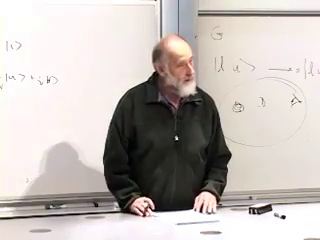
\includegraphics[width=0.66\textwidth]{lecture_07_figure_06.png}
\caption{從指定態向量轉向系綜描述的概念轉變。}
\lectureframe{01:29:43}
\end{figure}

若以機率\(\rho_i\)製備態\(|i\rangle\)，則密度算符為
\begin{equation}
\rho=\sum_i\rho_i|i\rangle\langle i|.
\end{equation}
在製備所用的基底中，
\begin{equation}
\rho=
\begin{pmatrix}
\rho_1&0&0&\cdots\\
0&\rho_2&0&\cdots\\
0&0&\rho_3&\cdots\\
\vdots&\vdots&\vdots&\ddots
\end{pmatrix}.
\end{equation}

\begin{figure}[htbp]
\centering
\includegraphics[width=0.68\textwidth]{lecture_07_figure_09.png}
\caption{對角密度矩陣及其歸一化條件。}
\lectureframe{01:32:12}
\end{figure}

其本徵值為實數且非負，而機率的歸一化條件則寫成
\begin{equation}
\operatorname{Tr}\rho=\sum_i\rho_i=1.
\end{equation}

令\(F\)為厄米可觀測量。系綜的期望值為
\begin{equation}
\langle F\rangle=\operatorname{Tr}(F\rho).
\end{equation}

\begin{figure}[htbp]
\centering
\includegraphics[width=0.68\textwidth]{lecture_07_figure_10.png}
\caption{跡的期望值\(\langle F\rangle=\operatorname{Tr}(F\rho)\)。}
\lectureframe{01:35:05}
\end{figure}

為了還原一般的加權平均，可在\(\rho\)的對角基底中計算跡，並插入單位算符的完備關係：
\begin{align}
\operatorname{Tr}(F\rho)
&=\sum_i\langle i|F\rho|i\rangle\\
&=\sum_{i,j}\langle i|F|j\rangle
               \langle j|\rho|i\rangle\\
&=\sum_i\rho_i\langle i|F|i\rangle.
\end{align}
因此，每個純態的期望值都乘上相應態被製備的機率，再加權求和。

跡具有循環性質
\begin{equation}
\operatorname{Tr}(AB)=\operatorname{Tr}(BA),
\end{equation}
即使\(A\)與\(B\)不對易也成立。因此，\(\operatorname{Tr}(F\rho)=\operatorname{Tr}(\rho F)\)。

\section{量子熵與延後揭曉的回報}

密度矩陣的熵為
\begin{equation}
S(\rho)=-\operatorname{Tr}(\rho\log\rho).
\end{equation}
對厄米正算符，諸如\(\log\rho\)這類函數是透過算符的本徵值來定義的。若
\begin{equation}
\rho=\sum_i\rho_i|i\rangle\langle i|,
\end{equation}
則
\begin{equation}
\log\rho=\sum_{\rho_i>0}(\log\rho_i)|i\rangle\langle i|,
\end{equation}
因此
\begin{equation}
S(\rho)=-\sum_i\rho_i\log\rho_i.
\end{equation}

\begin{figure}[htbp]
\centering
\includegraphics[width=0.68\textwidth]{lecture_07_figure_11.png}
\caption{將經典熵公式改寫為\(S=-\operatorname{Tr}(\rho\log\rho)\)。}
\lectureframe{01:41:25}
\end{figure}

已知純態的密度算符為
\begin{equation}
\rho_\psi=|\psi\rangle\langle\psi|,
\end{equation}
其本徵值為\(1,0,\ldots\)，因此\(S(\rho_\psi)=0\)。這並不表示對\(|\psi\rangle\)進行的每次測量都有確定結果，而是表示對於所製備的態，不存在額外的統計無知。另一個極端是
\begin{equation}
\rho=\frac{I}{d}
\qquad\Longrightarrow\qquad
S(\rho)=\log d,
\end{equation}
其中\(d=\dim\mathcal H\)。最大混合態對每個正交方向賦予相同權重。

現在已很接近糾纏的主題，但還沒真正展開。假設複合系統\(AB\)處於某個聯合態，而所有實驗都只在子系統\(A\)上進行。必定存在一個物件，能在忽略子系統\(B\)的情況下，重現對\(A\)所能取得的所有期望值。這個物件就是\(A\)的密度矩陣。若聯合態可以因式分解，\(A\)的密度矩陣便是純態，熵為零。若\(A\)與\(B\)糾纏，\(A\)的密度矩陣通常就是混合態，熵也不為零。如何構造這個約化密度矩陣並計算其熵，將留待下一講處理。
